% 行为学结果
% - [ ] 小鼠行为学结果
%   - [ ] 行为范式说明
% - [ ] 患者行为学结果
%   - [ ] 行为范式说明
%   - [ ] 韦伯定律
%   - [ ] 行为分布图
%   - [ ] 行为学提示所需的任务可能与增强学习相关

\section{小鼠的时间间隔预测行为}
为了探究视觉信息对小鼠的时间感知的影响,尤其是对视觉刺激所编码的时间的感知,
我们设计了连续周期性视觉刺激时间预测行为实验。通过耦连视觉刺激与小鼠舔水行为,
我们可以检测小鼠的舔水来推断小鼠内在的计时。

\subsection{规律刺激下的小鼠时间预测行为}
% 行为学范式示意图
% 一天舔水的示例
% 第一次舔水的分布曲线
% weber定律
我们选用了经过限水处理的野生型C57小鼠作为实验对象,每天包含5次连续的训练,
每次训练包含20个规律性的刺激。每次视觉刺激持续1秒,刺激间间隔为9秒;
每次刺激开始时小鼠均可以获得一定的水作为正向的反馈(图\ref{fig:mouse_behavior})。

为了评判小鼠在一天中的行为表现,我们将一天中小鼠舔水的行为时刻做了记录;
并以每次视觉刺激的开始作为原点,将前8秒和后2秒作为事件窗口对舔水行为做了分组。
同时,我们将不同组的行为以第一次舔水的时刻点做了排序(图\ref{fig:mouse_behavior})。
为了进一步比较不同天之间小鼠的行为表现,我们将第一次舔水的时刻点单独拿出来,
并对在视觉刺激之前发生的行为做了累计分布曲线(图\ref{fig:mouse_behavior})。
我们可以看到随着训练天数的增加,小鼠的舔水时刻向刺激开始的时间靠近。
前三天和后三天舔水的平均分布之间也存在统计学上的显著差异
(Kolmogorov–Smirnov检验,p值为$2.3 \times 10 ^ {-41}$), 提示了
小鼠在训练过程中存在着学习过程, 对刺激间时间间隔的感知准确度有所提高。

另一方面,我们也通过计算了小鼠行为学的韦伯系数(weber's fraction)
来检验小鼠对时间间隔的感知精确度(图\ref{fig:mouse_behavior})。
由于时间所限,我们未能对大量的老鼠
来做行为学;但我们依然能够看到随着训练时间的延长,小鼠行为学的韦伯系数
呈下降趋势。

综合小鼠的行为学结果来看,我们可以推断在连续周期性视觉刺激时间预测行为实验中,
小鼠对刺激间时间间隔的感知的精确度和准确度均有一定的提升,提示小鼠可能存在
学习过程;而小鼠大脑中神经元之间是否有发生动态的变化,还需要进一步的电生理实验
来验证。

\begin{figure}[h]
    \begin{center}

    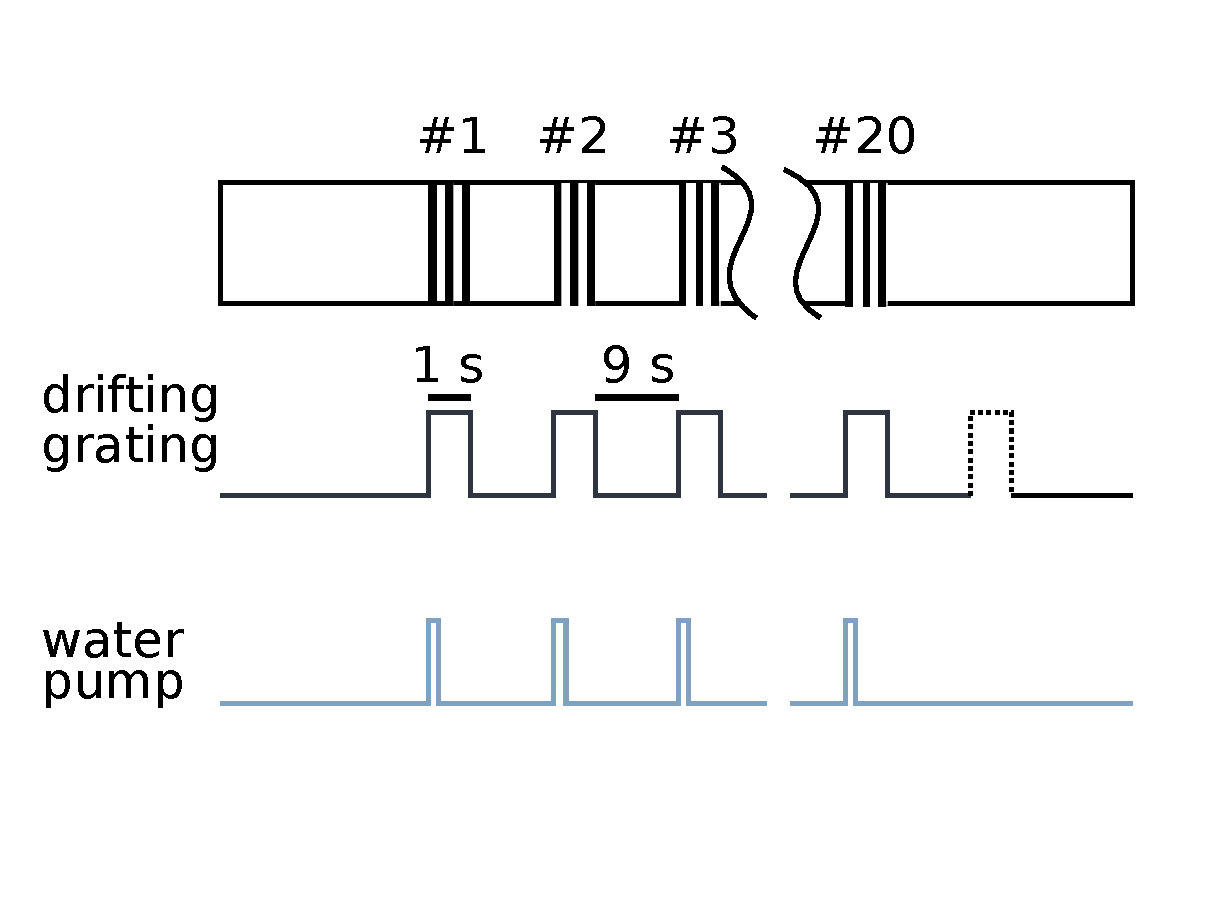
\includegraphics[width=0.45\textwidth]{src/figures/mouse_behavior_schema.pdf}
    ~
    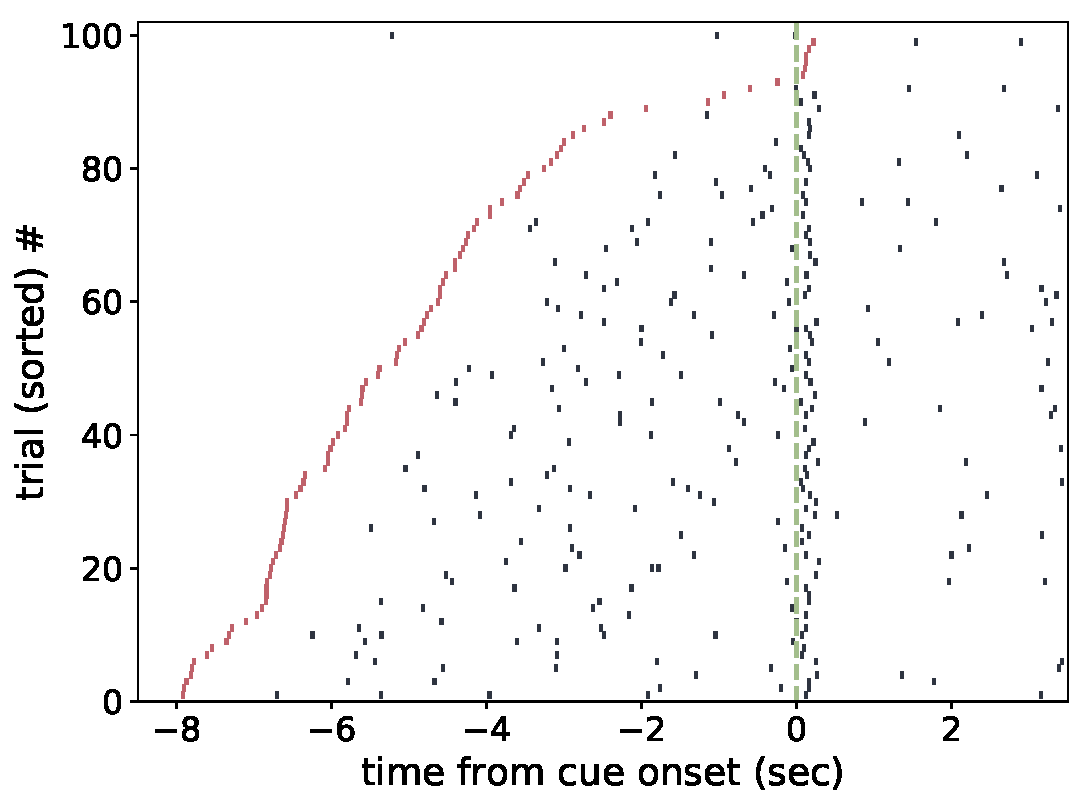
\includegraphics[width=0.45\textwidth]{src/figures/mouse_behavior_example.pdf}

    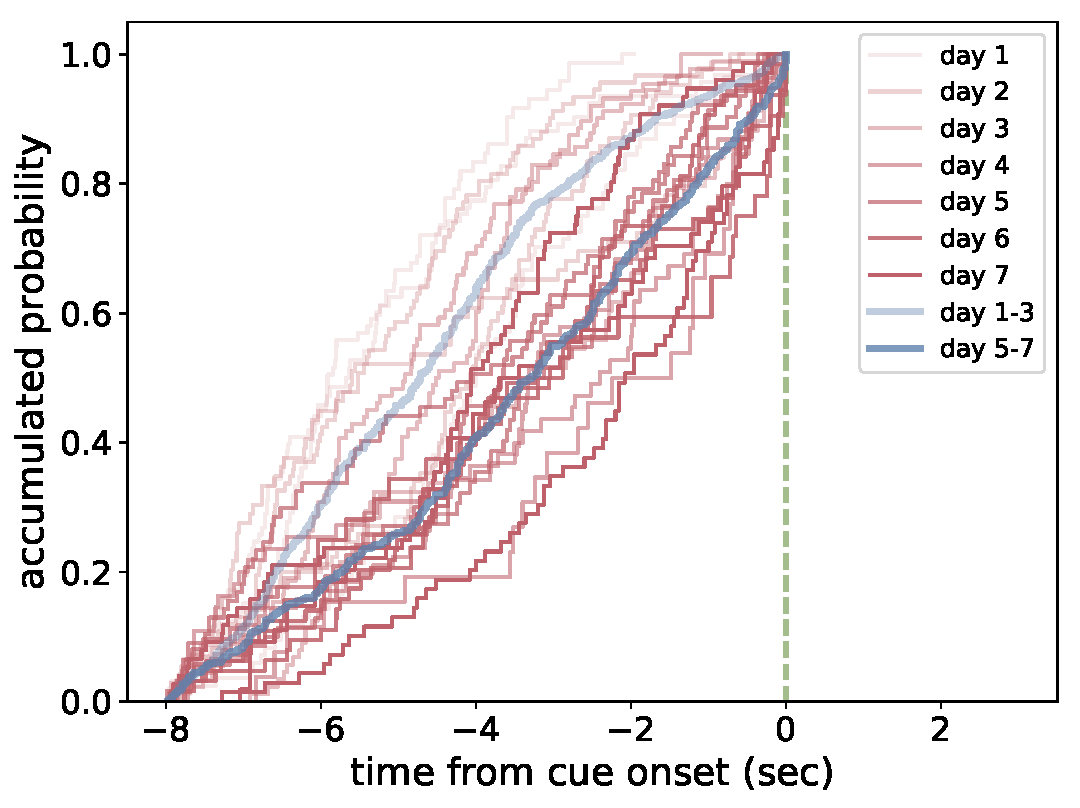
\includegraphics[width=0.45\textwidth]{src/figures/mouse_behavior_curve.pdf}
    ~
    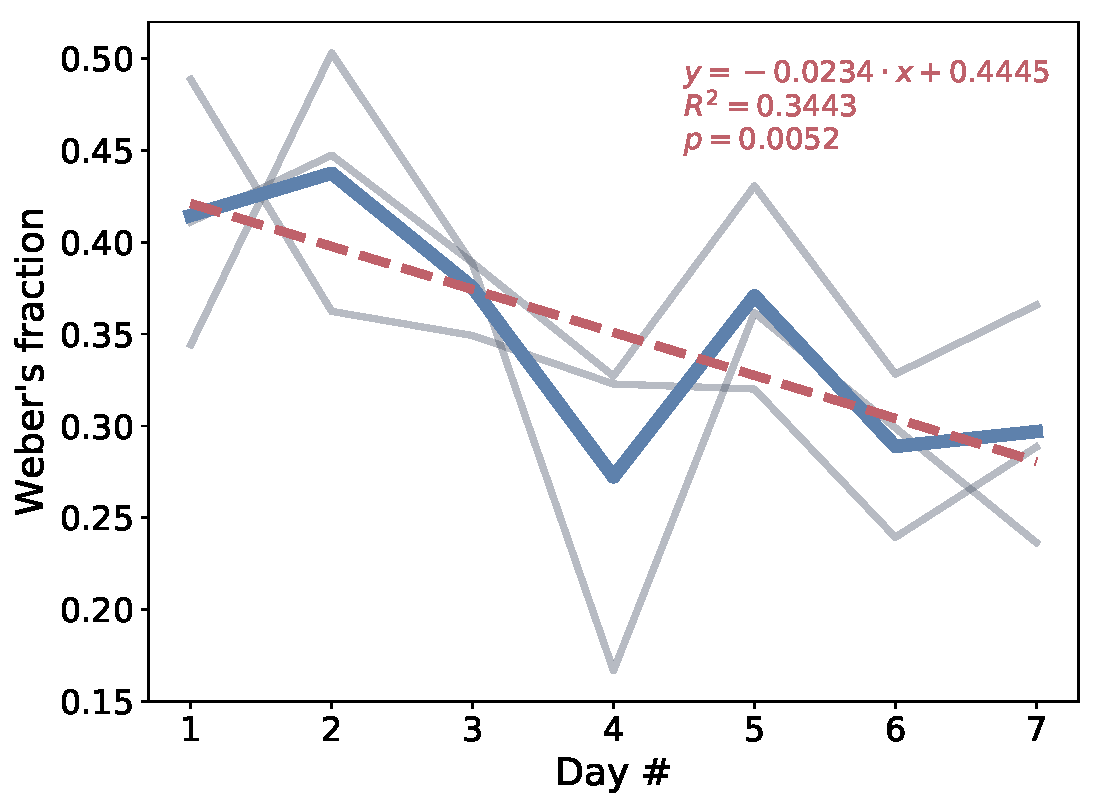
\includegraphics[width=0.45\textwidth]{src/figures/mouse_behavior_weber.pdf}
    \end{center}

    \caption{\textbf{规律刺激下的小鼠时间预测行为}\\
    一些额外的图注说明}
    \label{fig:mouse_behavior}
\end{figure}

%%%%%%%%%%%%%%%%%%%%%%%%%%%%%%%%%%%%%%%%%%%%%%%%%%%%%%%%%%%%%%%%
\section{患者的时间间隔预测行为}
为了让对人的实验结果与小鼠的实验结果可以

\subsection{心理测试范式}

\subsection{韦伯定律}

\subsection{轻拍手行为分布}

\subsection{行为结果所体现的可能的理论机制}

\begin{figure}[h]
    \centering
    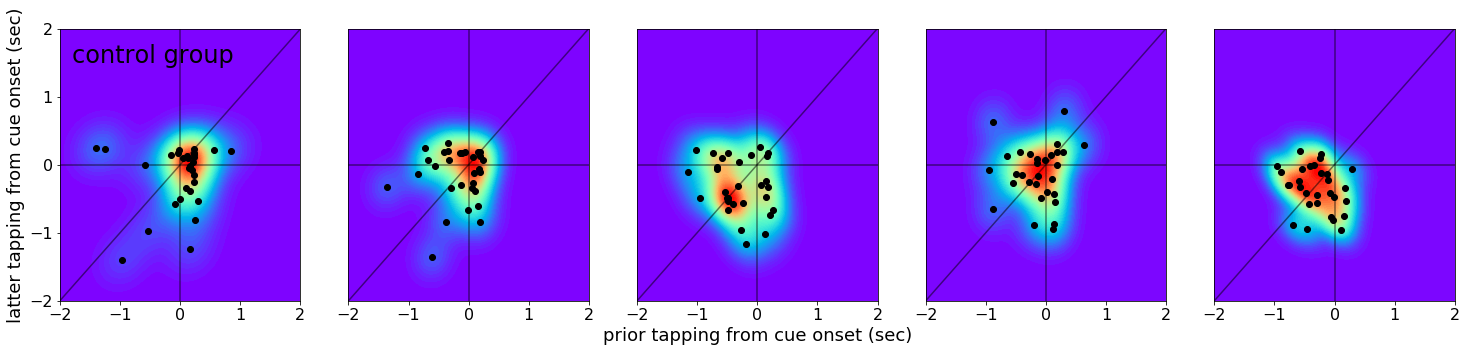
\includegraphics[width=0.9\textwidth]{src/figures/human_behavior_distribution_control.png}

    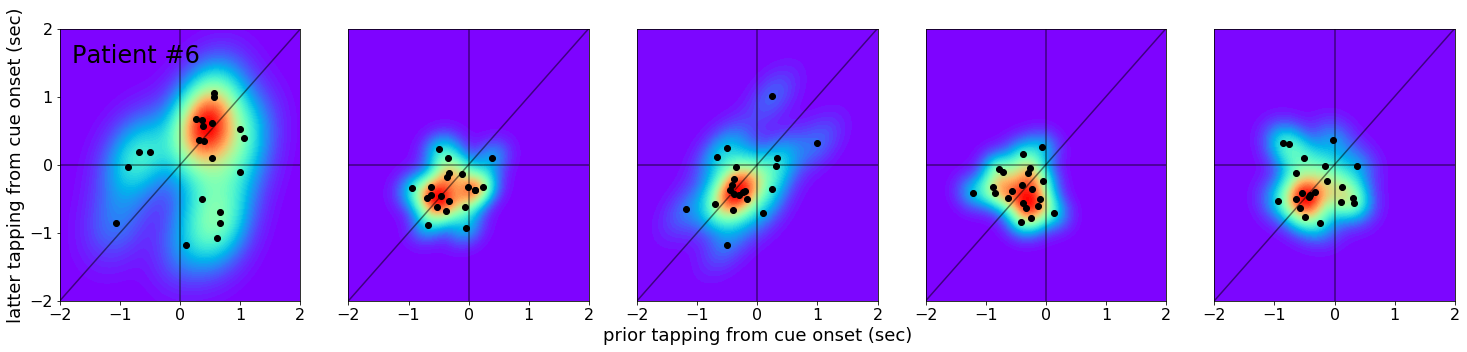
\includegraphics[width=0.9\textwidth]{src/figures/human_behavior_distribution_patient_6.png}

    \caption{规律刺激下的人的时间预测行为}
    \label{fig:human_behavior}
\end{figure}





